\documentclass{article}
\usepackage{graphicx} % Required for inserting images
\usepackage{minted} 
\usepackage[left=3cm, right=3cm, top=3cm, bottom=3cm]{geometry}
\usepackage{polski}
\usepackage[utf8]{inputenc}

\usepackage{booktabs}
\usepackage{pgfplots}

\title{Lista 3}
\author{Mateusz Kaczkowski}
\date{January 2026}

\begin{document}

\maketitle

Lista 3 polegała na napisaniu różnych algorytmów zachłannych oraz programowania dynamicznego. Algorytmy activity selector oraz huffman encoding należą to pierwszej z tych kategorii a cutrod oraz LSC do drugiej. Algorytmy te miały też wiele wariantów, często związane z rekurencją i iteracją, które zostały porównane pod względem prędkości.


\section{Problem Cięcia Pręta (Cut Rod)}
Problem polega na wyznaczeniu optymalnego sposobu pocięcia pręta o długości $n$ w celu maksymalizacji zysku. Porównano trzy podejścia:
\begin{itemize}
    \item \textbf{Wersja naiwna:} Rekurencyjne sprawdzanie wszystkich kombinacji.
    \item \textbf{Memoizacja:} Rekurencja z zapamiętywaniem wyników pośrednich.
    \item \textbf{Wersja iteracyjna:} Wypełnianie tablicy zysków metodą bottom-up.
\end{itemize}

\subsection{Najciekawsze fragmenty kodu}
Wersja iteracyjna algorytmu twoży listę najlepszych możliwych cen pręta o długości $i$ oraz najlepszego możliwego cięcia potrzebnego aby otrzymać ten wynik. Są one następnie wypełniane od długości 1 do $n$ i zwracane jako odpowiedź.
\begin{minted}{c}
tuple<int, vector<int>> cutRodIter(int n, int prices[]) {
    int* r = new int[n + 1]{ 0 };
    vector<int> rods(n, 1);

    for (int i = 1; i <= n; i++) {
        r[i] = prices[0] + r[i - 1];
        for (int j = 2; j <= i; j++)
            if (r[i] < prices[j - 1] + r[i - j]) {
                r[i] = prices[j - 1] + r[i - j];
                rods[i - 1] = j;
            }
    }
    int res = r[n];
    delete[] r;
    return make_tuple(res, rods);
}
\end{minted}

\subsection{Analiza wydajności}
Dla małych wielkości danych algorytm naiwny był jeszcze możliwy, ale dla dużych szybko stał się bezużyteczny ze względu na czas wykonania. Wersja iteracyjna zachowała stałą, mocną przewagę nad wersją rekurencyjną, co według mnie wynika z normalnych opóźnień związanych z wywołaniem funkcji rekurencyjnie oraz optymalizacji procesora dla pętli, szczególnie że wersja iteracyjna nie wygląda jakby podążała za spodziewaną wydajnością $n^2$, szczególnie dla wielkości mniejszej lub równej 50.

\begin{table}[h]
\centering
\large
\label{tab:wynikiCR}
\begin{tabular}{@{}|r||r|r|r|@{}}
\hline
Size & Naive & Memo & Iter \\
\hline
5   & 2,016     & 6,888    & 4,500   \\
10  & 36,836    & 6,844    & 5,152   \\
15  & 1240,140  & 13,540   & 6,660   \\
20  & 42324,176 & 21,996   & 7,556   \\
35  & N/A       & 27,324   & 12,548  \\
50  & N/A       & 30,108   & 13,276  \\
75  & N/A       & 57,124   & 17,240  \\
150 & N/A       & 229,108  & 40,788  \\
350 & N/A       & 1116,110 & 155,000 \\
700 & N/A       & 4485,860 & 560,104 \\
\hline
\end{tabular}
\caption{Czas wykonania algorytmów (µs) w zależności od rozmiaru danych}
\end{table}

\begin{figure}[h!]
\centering
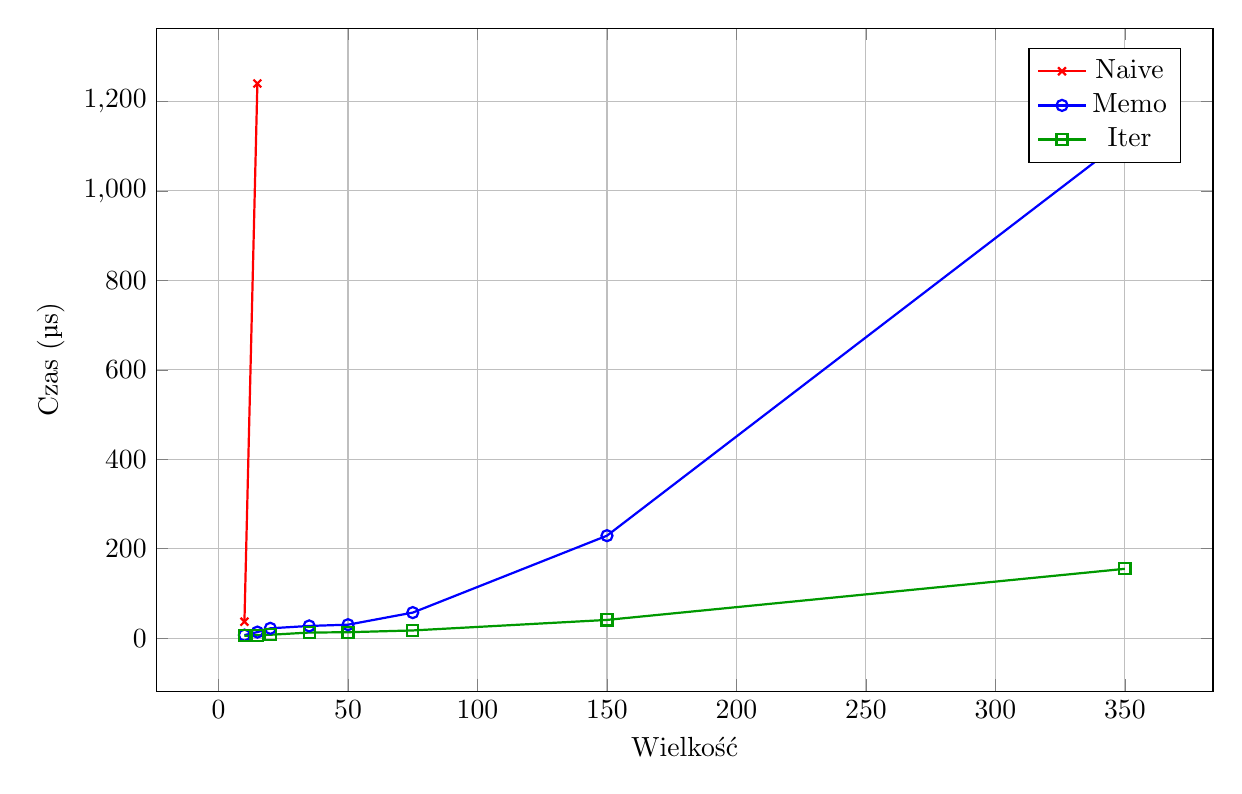
\begin{tikzpicture}
\begin{axis}[
    xlabel={Wielkość},
    ylabel={Czas (µs)},
    grid=major,
    legend pos=north east,
    width=15cm,
    height=10cm
]

\addplot[color=red, mark=x, thick] coordinates {
    (10, 36.836) (15, 1240.14)
};
\addlegendentry{Naive}

\addplot[color=blue, mark=o, thick] coordinates {
    (10, 6.844) (15, 13.54) (20, 21.996) (35, 27.324) 
    (50, 30.108) (75, 57.124) (150, 229.108) (350, 1116.11)
};
\addlegendentry{Memo}

\addplot[color=green!60!black, mark=square, thick] coordinates {
    (10, 5.152) (15, 6.66) (20, 7.556) (35, 12.548) 
    (50, 13.276) (75, 17.24) (150, 40.788) (350, 155)
};
\addlegendentry{Iter}

\end{axis}
\end{tikzpicture}
\end{figure}

\begin{figure}[h!]
\centering
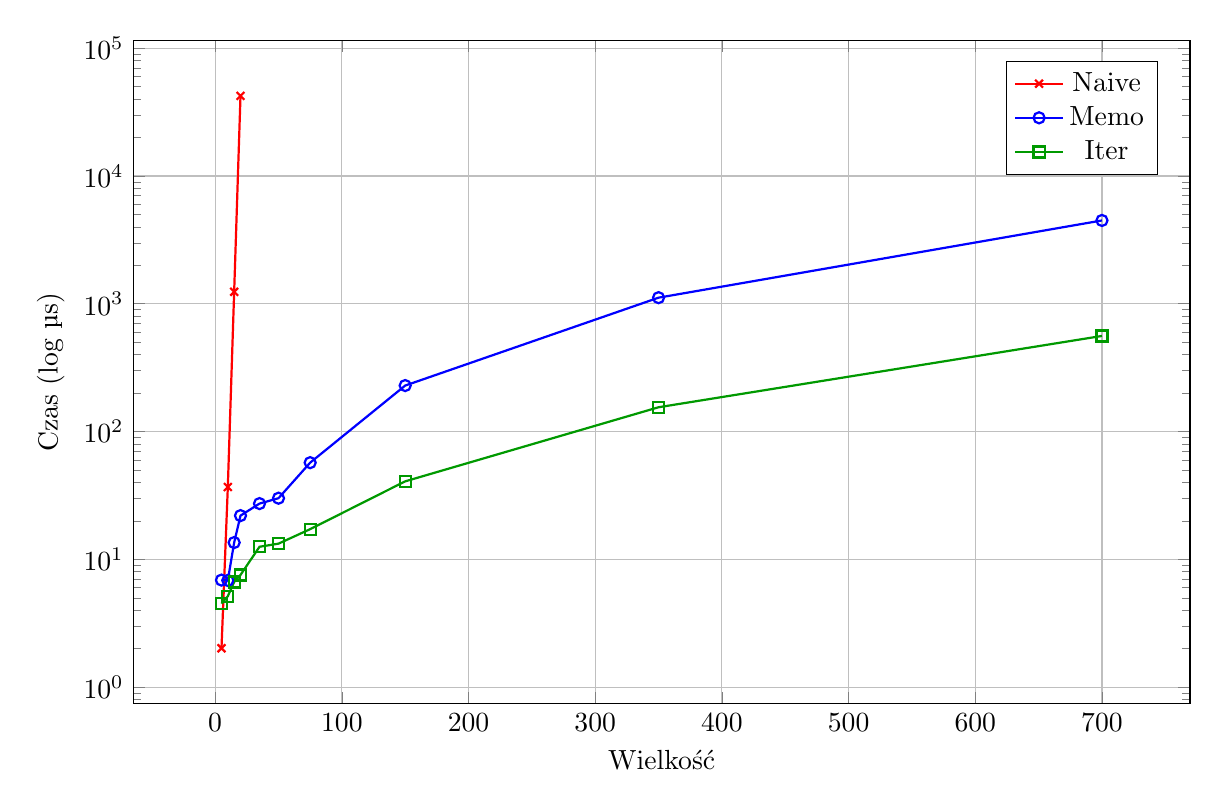
\begin{tikzpicture}
\begin{semilogyaxis}[
    xlabel={Wielkość},
    ylabel={Czas (log µs)},
    grid=major,
    legend pos=north east,
    width=15cm,
    height=10cm
]

\addplot[color=red, mark=x, thick] coordinates {
    (5, 2.016) (10, 36.836) (15, 1240.14) (20, 42324.176)
};
\addlegendentry{Naive}

\addplot[color=blue, mark=o, thick] coordinates {
    (5, 6.888) (10, 6.844) (15, 13.54) (20, 21.996) (35, 27.324) 
    (50, 30.108) (75, 57.124) (150, 229.108) (350, 1116.11) (700, 4485.86)
};
\addlegendentry{Memo}

\addplot[color=green!60!black, mark=square, thick] coordinates {
    (5, 4.5) (10, 5.152) (15, 6.66) (20, 7.556) (35, 12.548) 
    (50, 13.276) (75, 17.24) (150, 40.788) (350, 155) (700, 560.104)
};
\addlegendentry{Iter}

\end{semilogyaxis}
\end{tikzpicture}
\end{figure}

\newpage

\section{Najdłuższy Wspólny Podciąg (LCS)}

Algorytm wyznacza najdłuższy wspólny podciąg dwóch sekwencji przy użyciu $O(n^2)$ pamięci i czasu, uwzględniając odzyskiwanie rozwiązania. Napisany został on w wariantach rekurencyjnym i iteracyjnym, ale poza tym nie miały one większych różnic w designie.

\subsection{Najciekawsze fragmenty kodu}
Algorytm tworzy dwie tabele - wielkość najdłuższego dotąd znalezionego podciągu oraz strzałki pomagające jego odzyskanie. Są one następnie wypełniane po kolei, bazując na poprzednio ustalonych wartościach (założenie programowania dynamicznego). Aby odzyskać wynik tabela jest następnie przechodzona od końca po strzałkach, dodając odpowiednie elementy do podciągu.
\begin{minted}{c}
tuple<int, string> lcsIter(string& s1, string& s2) {
    int m = s1.size();
    int n = s2.size();

    vector<vector<int>> sizes(m + 1, vector<int>(n + 1, 0));
    vector<vector<int>> arrows(m + 1, vector<int>(n + 1, 0));

    for (int i = 1; i <= m; ++i) {
        for (int j = 1; j <= n; ++j) {
            if (s1[i - 1] == s2[j - 1]) {
                sizes[i][j] = sizes[i - 1][j - 1] + 1;
                arrows[i][j] = 3;
            }
            else if (sizes[i - 1][j] > sizes[i][j - 1]) {
                sizes[i][j] = sizes[i - 1][j];
                arrows[i][j] = 2;
            }
            else {
                sizes[i][j] = sizes[i][j - 1];
                arrows[i][j] = 1;
            }
        }
    }

    string lcs = "";
    int i = m, j = n;
    while (i > 0 && j > 0) {
        int arr = arrows[i][j];
        if (arr == 3) lcs = s1[i - 1] + lcs;
        if ((arr & 2) == 2) i--;
        if ((arr & 1) == 1) j--;
    }

    return make_tuple(sizes[m][n], lcs);
}
\end{minted}

\subsection{Analiza wydajności}

\begin{table}[h]
\centering
\large
\label{tab:wynikiLCS}
\begin{tabular}{@{}|r|r|r|@{}}
\hline
Size & Memo & Iter \\ 
\hline
10   & 0,2579  & 0,2327  \\
50   & 1,4016  & 1,3662  \\
100  & 4,2330  & 3,7790  \\
250  & 22,8205 & 20,0770 \\
400  & 60,3350 & 54,0543 \\
750  & 192,1040 & 161,8870 \\
1500 & 736,2690 & 627,8900 \\
\hline
\end{tabular}
\caption{Czas wykonania algorytmów (ms) w zależności od rozmiaru danych}
\end{table}

\newpage

\begin{figure}[h]
\centering
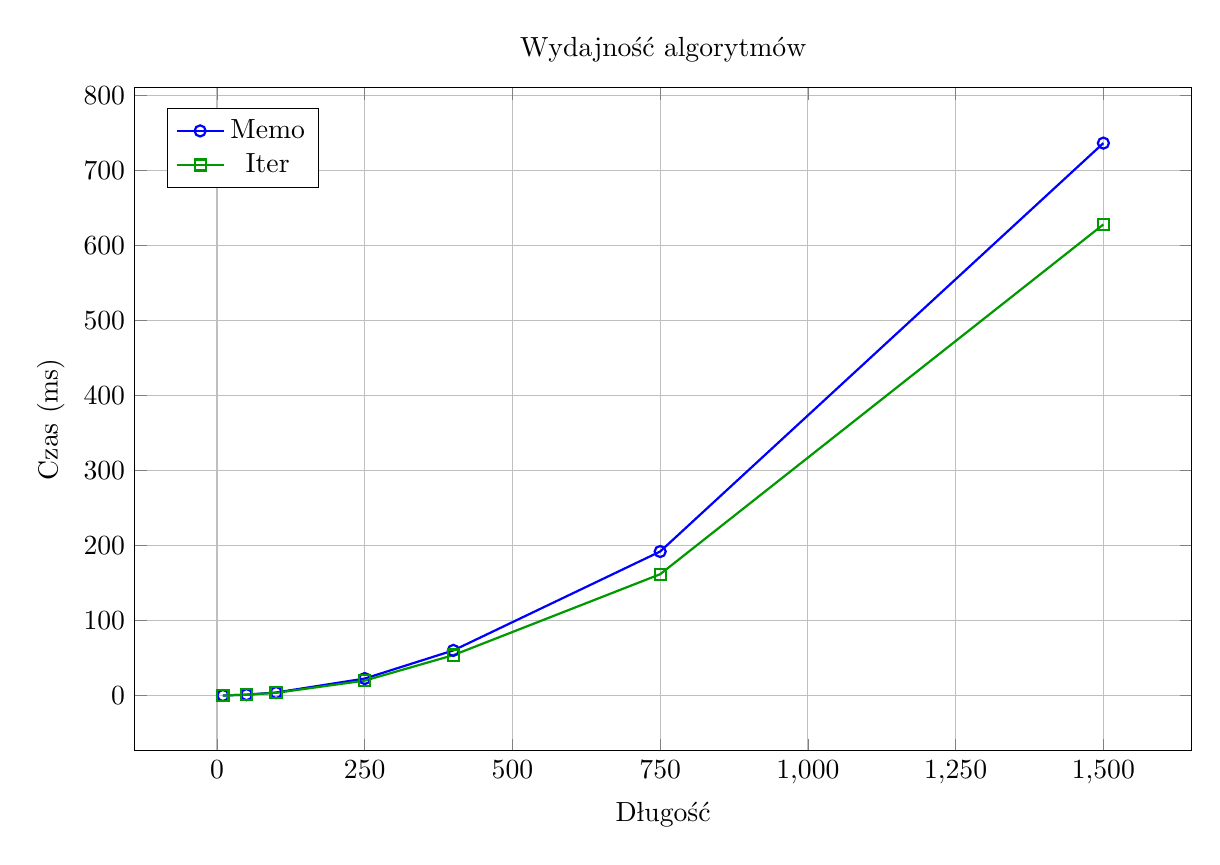
\begin{tikzpicture}
\begin{axis}[
    title={Wydajność algorytmów},
    xlabel={Długość},
    ylabel={Czas (ms)},
    grid=major,
    legend pos=north west,
    width=15cm,
    height=10cm,
    xtick={0, 250, 500, 750, 1000, 1250, 1500},
]

\addplot[color=blue, mark=o, thick] coordinates {
    (10, 0.2579) (50, 1.4016) (100, 4.233) (250, 22.8205) 
    (400, 60.335) (750, 192.104) (1500, 736.269)
};
\addlegendentry{Memo}

\addplot[color=green!60!black, mark=square, thick] coordinates {
    (10, 0.2327) (50, 1.3662) (100, 3.779) (250, 20.077) 
    (400, 54.0543) (750, 161.887) (1500, 627.89)
};
\addlegendentry{Iter}

\end{axis}
\end{tikzpicture}
\caption{Wykres porównawczy czasów wykonania algorytmów Memo i Iter.}
\end{figure}

\section{Activity Selector}
Activity Selector to algorytm wyszukujący największy zbiór rozłącznych przedziałów wziętych z danej na wejściu listy. Zachłanne wersje tego algorytmu zakładały już posortowane dane wejściowe.
\begin{itemize}
    \item \textbf{Iteracyjna:} Zachłanne wypełnianie tablicy dla danych posortowanych po końcu aktywności.
    \item \textbf{Rekurencja:} Rekurencyjna wersja pętli dla danych posortowanych po końcu aktywności.
    \item \textbf{Iteracyjna odwrócona:} Zachłanne wypełnianie tablicy dla danych posortowanych po początku aktywności.
    \item \textbf{Rekurencja odwrócona:} Rekurencyjna wersja pętli dla danych posortowanych po początku aktywności.
    \item \textbf{Programowanie dynamiczne:} Wypełnianie tablicy map najlepszymi wyborami aktywności metodą bottom-up. Wolniejsza i nadmiernie skomplikowana metoda dla problemu sformułowanego w zadaniu, ale może stanowić bazę dla innych rozwiązań nie dających rozwiązać się zachłannie.
\end{itemize}

\subsection{Najciekawsze fragmenty kodu}
Jedyny kod z tej listy który wydał mi się naprawdę ciekawy, szczególnie że nie ma on standardowych, przygotowanych rozwiązań. Algorytm opiera się na dwuwymiarowej tablicy, której kolumny nie sąsiadują ze sobą pod względem indeksów. Rozwiązałem to przy pomocy wektora map. Rzędy tej tabeli oznaczają rozwiązania dla aktywności od 0 do indeksu $i$, a kolumny to rozwiązania dla aktywności kończących się przed czasem $end$. Ta tabela jest następnie rekurencyjnie wypełniana dla kolejnych $i$, zakładając jego dodanie oraz odrzucenie, a następnie biorąc większy wynik.
\begin{minted}
set<int> activitySelectionDynamic(int i, int end, vector<pair<int, int>> &activities, vector<map<int, set<int>>> &solution) {
    int n = activities.size();
    if (i == n) return {};
    set<int> v1, v2;
    if (solution[i].contains(end)) return solution[i][end];

    v1 = activitySelectionDynamic(i + 1, end, activities, solution);
    if (activities[i].first >= end) {
        v2 = activitySelectionDynamic(i + 1, activities[i].second, activities, solution);
        v2.insert(i);
    }
    return solution[i][end] = v1.size() > v2.size() ? v1 : v2;
}
set<int> activitySelectionDynamic(vector<pair<int, int>> activities) {
    vector<map<int, set<int>>> sol(activities.size());
    activitySelectionDynamic(0, 0, activities, sol);
    return sol[0][0];
}
\end{minted}

\subsection{Analiza wydajności}


\begin{table}[h]
\centering
\label{tab:wynikiAS}
\large
\begin{tabular}{@{}|r|r|r|r|r|r|@{}}
\hline
Size & Dyna & Rec & Iter & RecRev & IterRev \\ 
\hline
10   & 959,98    & 21,60   & 15,20   & 18,73   & 12,21   \\
100  & 132379,96 & 201,06  & 106,39  & 188,35  & 106,50  \\
250  & N/A       & 491,58  & 282,26  & 524,49  & 278,92  \\
500  & N/A       & 988,42  & 583,22  & 1003,75 & 570,16  \\
1000 & N/A       & 2063,30 & 1243,51 & 2078,16 & 1193,51 \\
\hline
\end{tabular}
\end{table}

\begin{figure}[h!]
\centering
\caption{Wykres w skali logarytmicznej.}
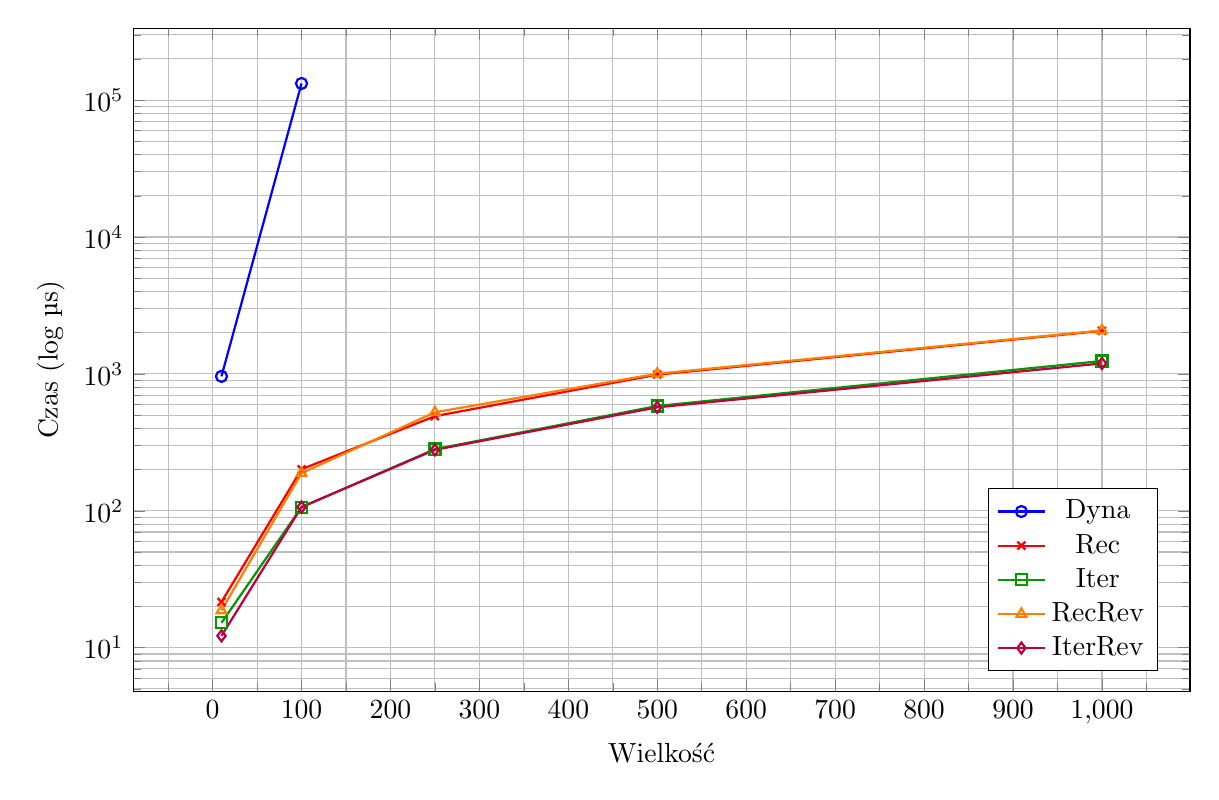
\begin{tikzpicture}
\begin{semilogyaxis}[
    xlabel={Wielkość},
    ylabel={Czas (log µs)},
    grid=both, 
    minor tick num=1,
    legend pos=south east,
    width=15cm,
    height=10cm,
]

% Dyna
\addplot[color=blue, mark=o, thick] coordinates {
    (10, 959.98) (100, 132379.96)
};
\addlegendentry{Dyna}

% Rec
\addplot[color=red, mark=x, thick] coordinates {
    (10, 21.6) (100, 201.06) (250, 491.58) (500, 988.42) (1000, 2063.3)
};
\addlegendentry{Rec}

% Iter
\addplot[color=green!60!black, mark=square, thick] coordinates {
    (10, 15.2) (100, 106.39) (250, 282.26) (500, 583.22) (1000, 1243.51)
};
\addlegendentry{Iter}

% RecRev
\addplot[color=orange, mark=triangle, thick] coordinates {
    (10, 18.73) (100, 188.35) (250, 524.49) (500, 1003.75) (1000, 2078.16)
};
\addlegendentry{RecRev}

% IterRev
\addplot[color=purple, mark=diamond, thick] coordinates {
    (10, 12.21) (100, 106.5) (250, 278.92) (500, 570.16) (1000, 1193.51)
};
\addlegendentry{IterRev}

\end{semilogyaxis}
\end{tikzpicture}
\end{figure}

\begin{figure}[h!]
\centering
\caption{Wykres w skali liniowej.}
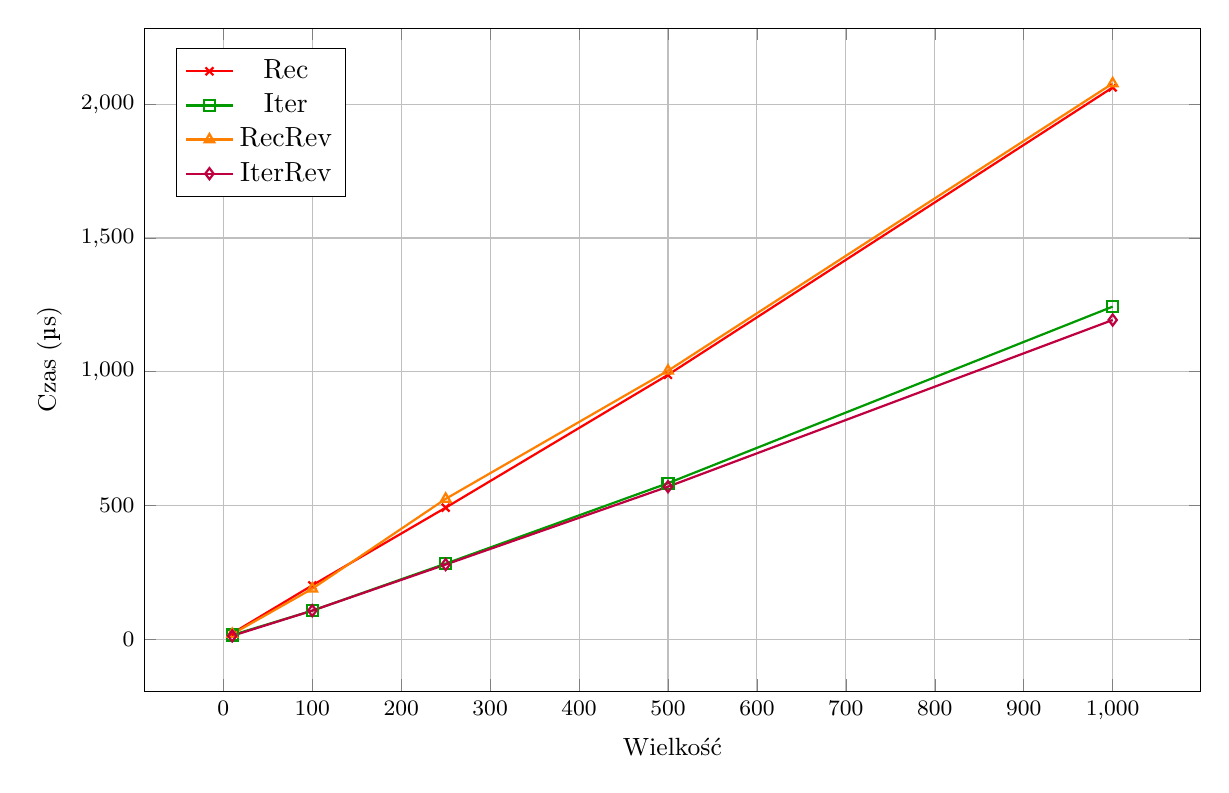
\begin{tikzpicture}
\begin{axis}[
    xlabel={Wielkość},
    ylabel={Czas (µs)},
    grid=major,
    legend pos=north west,
    width=15cm,
    height=10cm,
    tick label style={font=\footnotesize},
    label style={font=\small},
]

% Rec
\addplot[color=red, mark=x, thick] coordinates {
    (10, 21.6) (100, 201.06) (250, 491.58) (500, 988.42) (1000, 2063.3)
};
\addlegendentry{Rec}

% Iter
\addplot[color=green!60!black, mark=square, thick] coordinates {
    (10, 15.2) (100, 106.39) (250, 282.26) (500, 583.22) (1000, 1243.51)
};
\addlegendentry{Iter}

% RecRev
\addplot[color=orange, mark=triangle, thick] coordinates {
    (10, 18.73) (100, 188.35) (250, 524.49) (500, 1003.75) (1000, 2078.16)
};
\addlegendentry{RecRev}

% IterRev
\addplot[color=purple, mark=diamond, thick] coordinates {
    (10, 12.21) (100, 106.5) (250, 278.92) (500, 570.16) (1000, 1193.51)
};
\addlegendentry{IterRev}

\end{axis}
\end{tikzpicture}
\end{figure}

\newpage

\section{Huffman}
Kodowanie Huffmana to algorytm kompresji danych oparty o drzewo przydzielające najczęściej występującym znakom najkrótsze kody. Jego czas skaluje się liniowo z długością tekstu, więc testy czasu nie mają specjalnie sensu. Zamiast tego porównałem wielkość kompresji kodowań binarnych i ternarnych. Dla tekstu o długości 8625 znaków, zapisanie go formacie ASCII wymagane byłoby 69000 bitów, ale jego kodowanie Huffmana potrzebuje ich jedynie 36605, a wersja ternarna tylko 23382 tritów. Zgodnie z oczekiwaniami $\frac{36605}{23382} = 1.5655 \approx 1.5849 = \log_{2}(3)$. 
\section{Wnioski}
\begin{enumerate}
    \item \textbf{Cut Rod:} Algorytm iteracyjny jest znacząco szybszy od memoizacji , co wynika prawdopodobnie wynika z wywołań stosu rekurencji. Argortym naiwny jest nieefektywny nawet dla bardzo małych danych.
    \item \textbf{LCS:} Różnice między memoizacją a iteracją są mniejsze niż w przypadku Cut Rod, jednak podejście iteracyjne pozostaje o ok. 15\% wydajniejsze.
    \item \textbf{Activity Selector:} Podejście zachłanne iteracyjne pozostaje lepsze od rekurencyjnego pod względem wydajności dla danych posortowanych, niezależnie od kierunku sortowania. Programowanie dynamiczne w tym przypadku drastycznie gorsze, jednak pozwala na oddanie znacznie większej ilości ograniczeń jako modyfikacje problemu. 
    \item \textbf{Kod C++:} Ogromne znaczenie w wydajności wszystkich algorytmów miały detale kodu w c++, takie jak przekazywanie odniesienia do wektora zamiast samego wektora, czy odpowiednie używanie wskaźników. Jest duża szansa że przedstawione tu algorytmy można byłoby znacznie zoptymalizować pisząc je zgodnie z praktykami c++ oraz znajomością architektury procesora. 
\end{enumerate}

\end{document}
